
\chapter{Registration}

\piccaption[2]{Image registration is the task of finding a spatial transform
  mapping on image into another.\label{fig:ImageRegistrationConcept}}
\parpic(8cm,3cm)[r]{\includegraphics[width=8cm]{ImageRegistrationConcept.eps}}
  
This chapter introduces the functionalities offered by Insight for performing
image registration. Image registration is the process in which we determine the
spatial transform that maps points from one image to homologous points on the
object in the second image. This concept is schematically represented in Figure
\ref{fig:ImageRegistrationConcept}. In the toolkit, registration is performed
within a framework of pluggable components that can easily be interchanged.
This flexibility means that a combinatorial variety of registration methods can
be created, allowing the user to pick and choose the right tools for the
application.


\section{Registration Framework}
The components of the registration framework and their interconnections 
are shown in Figure \ref{fig:RegistrationComponents}. The basic
input data to the registration process are two images: one
is defined as the \emph{Fixed} image $f(\bf{X})$ and the other defined as the
\emph{Moving} image $m(\bf{X})$. Registration is treated as an optimization problem
with the goal of finding the spatial mapping that will bring the moving image into 
alignment with the fixed or target image.

\begin{figure}
\center
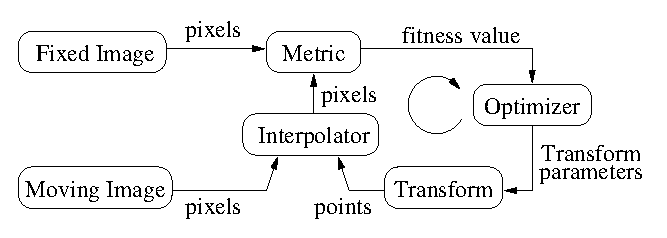
\includegraphics[width=12cm]{RegistrationComponentsDiagram.eps}
\caption{The basic components of the registration framework are two input images,
a transform, a metric, an interpolator and an optimizer.}
\label{fig:RegistrationComponents}
\end{figure}

The \emph{Transform} component $T(\bf{X})$ represents the spatial mapping of points 
from the fixed image space to points in the moving image space. Note that this 
definition is inverse to the usual view of image transformation. Using the
\emph{inverse} transform is typical in registration as it avoids the potential
problems of "holes" with forward transform. The \emph{Interpolator} is used to
evaluate moving image intensity at non-grid positions. The \emph{Metric} component
$S(f,m \circ T)$ provides a measure of how well the fixed image is matched by 
the transformed moving image. This measure forms the quantitative criterion to be optimized 
by the \emph{Optimizer} over the search space defined by the parameters of the 
\emph{Transform}.

The various components available in the toolkit will be described in later sections.
First we begin with a simple registration example.

\section{Hello World Registration}
\label{sec:IntroductionImageRegistration}
\input{ImageRegistration1.tex}


\section{Transforms}
\label{sec:Transforms}
In the toolkit, \code{itk::Transform} objects encapsulates the mapping of
points, vectors and covariant vectors from an input space to an output space.
The distinction between points, vectors and covariant vectors has already
been discussed in Chapter \ref{sec:DataRepresentation}. If a transform is
invertible, back transform methods are also provided. Currently, 
ITK provide a variety of transfroms from simple translation, rotation and 
scaling to general affine and kernel transforms. Note that, although we
discuss transforms in context registration in this section, transforms
are general and can used for other applications. Some of the commonly used 
transforms will be discussed in detail later in this section.

Typically, each transform type several methods are provided for setting
the parameters. For example, \code{Euler2DTransform} provide methods for
separatedly setting the offset, the angle, and the entire rotation matrix.
However, for use in the registration framework, the parameters must also
be represented by a flat \code{Array<double>} to allow communication
with generic optimizers. In the case of \code{Euler2DTransform}, the transform
is also defined by three doubles: the first representing the angle and 
the last two the offset. The a description of the parameters and their
ordering is documented in the header file of each transform.

Another requirement of the registration framework is the of the
transformation Jacobian. In general, metrics require the knowledge of 
the Jacobian in order to compute the metric derivatives. 
The Jacobian is a matrix whose element are the partial derivatives of the 
output point with respect to the array of parameters that defines the 
transform:

\begin{equation}
J=\left[ \begin{array}{cccc}
\frac{\partial x_{1}}{\partial p_{1}} & 
\frac{\partial x_{2}}{\partial p_{1}} & 
\cdots  & \frac{\partial x_{n}}{\partial p_{1}}\\
\frac{\partial x_{1}}{\partial p_{2}} & 
\frac{\partial x_{2}}{\partial p_{2}} & 
\cdots  & \frac{\partial x_{n}}{\partial p_{2}}\\
\vdots  & \vdots  & \ddots  & \vdots \\
\frac{\partial x_{1}}{\partial p_{m}} & 
\frac{\partial x_{2}}{\partial p_{m}} & 
\cdots  & \frac{\partial x_{n}}{\partial p_{m}}
\end{array}\right]
\end{equation}
 

\subsection{Identity Transform}
\label{sec:IdentityTransform}
\begin{array}{rr}
\bf{Behavior} & 
Maps every point to itself, every vector to itself and every covariant vector to itself. \\
\bf{No. of parameters} & 
0 \\
\bf{Parameter Ordering} & 
\\
\bf{Restrictions} &
Only defined when the input and output space has the same number of dimensions. \\
\end{array}


\subsection{Translation Transform}
\label{sec:TranslationTransform}
\begin{array}{rr}
\bf{Behavior} & 
Represents a simple translation of points in the input space
and has no effect on vectors or covariant vectors. \\
\bf{No. of parameters} & 
Same as the input space dimension.\\
\bf{Parameter Ordering} & 
The i-th parameter represents the translation in the i-th dimension. \\
\bf{Restrictions} &
Only defined when the input and output space has the same number of dimensions. \\
\end{array}
 
\subsection{ScaleTransform}
\label{sec:ScaleTransform}
\begin{array}{rr}
\bf{Behavior} & 
Represents a simple scaling of the vector space. Each componet of a point, vector
or covariant vector is multiplied by the user defined scaling factor.\\
\bf{No. of parameters} & 
Same as the input space dimension. \\
\bf{Parameter Ordering} & 
The i-th parameter represents the scaling in the i-th dimension. \\
\bf{Restrictions} &
Only defined when the input and output space has the same number of dimensions. \\
\end{array}

\subsection{Euler2DTransform}
\label{sec:Euler2DTransform}
\begin{array}{rr}
\bf{Behavior} & 
Represents a 2D rotation and a 2D translation. Note that the translation
componet has no effect on the transformation of vectors and covariant vectors. \\
\bf{No. of parameters} & 
3\\
\bf{Parameter Ordering} & 
The first parameter is the angle in radian and the last two parameters
are the translation in each each dimension. \\
\bf{Restrictions} &
Only defined for two-dimensional input and output spaces. \\
\end{array}

\subsection{Similarity2DTransform}
\label{sec:Similarity2DTransform}
\begin{array}{rr}
\bf{Behavior} & 
Represents a 2D rotation, homogenous scaling and a 2D translation. Note that the translation
componet has no effect on the transformation of vectors and covariant vectors. \\
\bf{No. of parameters} & 
4\\
\bf{Parameter Ordering} & 
The first parameter is the angle in radian, the second the scaling factor for all
dimension and the last two parameters are the translation in each dimension. \\
\bf{Restrictions} &
Only defined for two-dimensional input and output spaces. \\
\end{array}

\subsection{QuaternionRigidTransform}
\begin{array}{rr}
\bf{Behavior} & 
Represents a 3D rotation and a 3D translation. The rotation is specified
as a quaternion, defined by a vector of four numbers $\bf{q}$.
The relationship between quaternion and rotation about vector $\bf{n}$ by
angle $\theta$ is as follows:
\[ \bf{q} = (\bf{n}\sin(\theta/2), \cos(\theta/2))\]
Note that if the quaternion is not of unit length, scaling will also result. \\
\bf{No. of parameters} & 
7\\
\bf{Parameter Ordering} & 
The first four parameters defines the quaternion and the last three parameters
the translation in each dimension. \\
\bf{Restrictions} &
Only defined for three-dimensional input and output spaces. \\
\end{array}

\subsection{VersorRigid3DTransform}
\label{sec:VersorRigid3DTransform}
\begin{array}{rr}
\bf{Behavior} & 
Represents a 3D rotation and a 3D translation. The rotation is specified 
a versor or unit quaternion, defined by a vector of three numbers $\bf{q}$.
These three numbers corresponds to the first three components of a quaternion.
The fourth component of the quaternion derived such that the quaternion
is of unit length.
\\
\bf{No. of parameters} & 
6\\
\bf{Parameter Ordering} & 
The first three parameters defines the versor and the last three parameters
the translation in each dimension. \\
\bf{Restrictions} &
Only defined for three-dimensional input and output spaces. \\
\end{array}

\subsection{AffineTransform}
\label{sec:AffineTransform}
\begin{array}{rr}
\bf{Behavior} & 
Represents an affine transform composed of rotation, scaling, shearing and
translation. The transform is specified by a $N \times N$ matrix and
a $N \times 1$ vector where $N$ is space dimension. \\
\bf{No. of parameters} & 
$(N+1) \times N$\\
\bf{Parameter Ordering} & 
The first $N \times N$ parameters defines the matrix in column-major order
(where the column index varies the fastest).
The last $N$ parameters defines the translate for each dimension. \\
\bf{Restrictions} &
Only defined when the input and output space have the same dimension. \\
\end{array}





\section{Interpolators}
\label{sec:Interpolators}
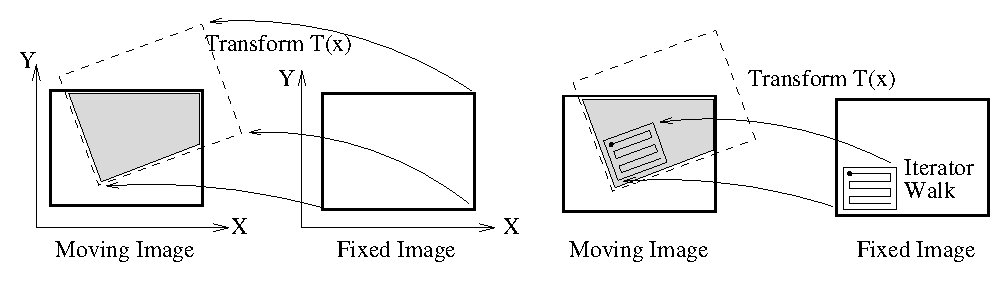
\includegraphics{ImageOverlap.eps}

An Image A is mapped over an image B by using a Transform


\subsection{Iterator Walking over a Region}

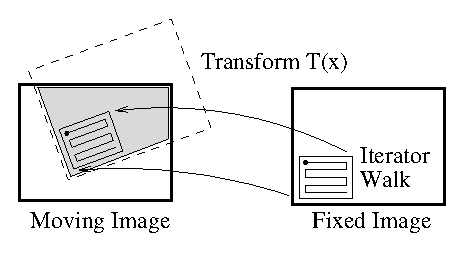
\includegraphics{ImageOverlapIterator.eps} 

An Iterator walking over a region of
B gets mapped on top of a blue region of A

\subsection{Need for an Interpolator}

The positions of the iterator are mapped
on non-grid positions in the image A 


\includegraphics{ImageOverlapInterpolator.eps}

An interpolation is needed for estimating
the value of the image A at these non-grid positions.


\subsection{Overlaped regions }


\includegraphics{ImageOverlapedRegions.eps}

Image metrics perform the computation over the intersection of a region in
image A and the map of a region in image B.




\section{Metrics}
\label{sec:Metrics}
%
%  This file is included by Registration.tex
%
%
%

\index{itk::Image\-To\-Image\-Metricv4}

In ITK, \doxygen{ImageToImageMetricv4} objects quantitatively measure how well
the transformed moving image fits the fixed image by comparing the gray-scale
intensity of the images. These metrics are very flexible and can work with any
transform or interpolation method and do not require reduction of the
gray-scale images to sparse extracted information such as edges.

The metric component is perhaps the most critical element of the registration
framework. The selection of which metric to use is highly dependent on the
registration problem to be solved. For example, some metrics have a large
capture range while others require initialization close to the optimal
position.  In addition, some metrics are only suitable for comparing images
obtained from the same imaging modality, while others can handle
inter-modality comparisons.
Unfortunately, there are no clear-cut rules as to how to choose a metric.

\index{itk::Image\-To\-Image\-Metricv4!GetValue()}
\index{itk::Image\-To\-Image\-Metricv4!GetDerivatives()}
\index{itk::Image\-To\-Image\-Metricv4!GetValueAndDerivatives()}

The matching Metric class controls most parts of the registration process
since it handles fixed, moving and virtual images as well as fixed and moving
transforms and interpolators.  The method \code{GetValue()} can be used to
evaluate the quantitative criterion at the transform parameters specified in
the argument.  Typically, the metric samples points within a defined region
of the virtual lattice.  For each point, the corresponding fixed and moving
image positions are computed using the fixed initial transform and the moving
transform with the specified parameters. Then, the fixed and moving interpolators
are used to compute the fixed and moving image's intensities at the mapped
positions. Details on this mapping are illustrated in Figures
\ref{fig:ImageOverlapIterator} and \ref{fig:ImageOverlapInterpolator} assuming
that virtual lattice is the same as the fixed image lattice, which is usually the
case in practice.

The metrics also support region-based evaluation. The \code{SetFixedImageMask()} and
\code{SetMovingImageMask()} methods may be used to restrict evaluation of the metric
within a specified region. The masks may be of any type derived from \doxygen{SpatialObject}.

Besides the measure value, gradient-based optimization schemes also require
derivatives of the measure with respect to each transform parameter. The
methods \code{GetDerivatives()} and \code{GetValueAndDerivatives()} can be
used to obtain the gradient information.


The following is the list of metrics currently available in ITKv4 registration framework:
\begin{itemize}
\item Mean squares\\ \doxygen{MeanSquaresImageToImageMetricv4}
\item Correlation \\ \doxygen{CorrelationImageToImageMetricv4}
\item Mutual information by Mattes \\ \doxygen{MattesMutualInformationImageToImageMetricv4}
\item Joint histogram mutual information \\ \doxygen{JointHistogramMutualInformationHistogramImageToImageMetricv4}
\item Demons metric \\ \doxygen{DemonsImageToImageMetricv4}
\item ANTS neighborhood correlation metric \\ \doxygen{ANTSNeighborhoodCorrelationImageToImageMetricv4}
\end{itemize}

Also, in case you are interested in using the legacy ITK registration framework,
the following is the list of metrics currently available in ITKv3:
\begin{itemize}
\item Mean squares\\ \doxygen{MeanSquaresImageToImageMetric}
\item Normalized correlation \\ \doxygen{NormalizedCorrelationImageToImageMetric}
\item Mean reciprocal squared difference \\ \doxygen{MeanReciprocalSquareDifferenceImageToImageMetric}
\item Mutual information by Viola and Wells \\ \doxygen{MutualInformationImageToImageMetric}
\item Mutual information by Mattes \\ \doxygen{MattesMutualInformationImageToImageMetric}
\item Kullback Liebler distance metric by Kullback and Liebler \\ \doxygen{KullbackLeiblerCompareHistogramImageToImageMetric}
\item Normalized mutual information \\ \doxygen{NormalizedMutualInformationHistogramImageToImageMetric}
\item Mean squares histogram \\ \doxygen{MeanSquaresHistogramImageToImageMetric}
\item Correlation coefficient histogram \\ \doxygen{CorrelationCoefficientHistogramImageToImageMetric}
\item Cardinality Match metric \\ \doxygen{MatchCardinalityImageToImageMetric}
\item Kappa Statistics metric\\ \doxygen{KappaStatisticImageToImageMetric}
\item Gradient Difference metric \\ \doxygen{GradientDifferenceImageToImageMetric}
\end{itemize}

In the following sections, we describe the ITKv4 metric types in detail.
You can check ITK descriptions in doxygen for details about ITKv3 metric classes.

For ease of notation, we will refer to the fixed image $f(\bf{X})$
and transformed moving image $(m \circ T(\bf{X}))$ as images $A$ and $B$.

\subsection{Mean Squares Metric}
\label{sec:MeanSquaresMetricv4}
\index{itk::Mean\-Squares\-Image\-To\-Image\-Metricv4}

The \doxygen{MeanSquaresImageToImageMetricv4} computes the mean squared
pixel-wise difference in intensity between image $A$ and $B$ over a user
defined region:

\begin{equation}
MS(A,B) = \frac{1}{N} \sum_{i=1}^N \left( A_i - B_i \right)^2
\end{equation}
\begin{center}
$A_i$ is the i-th pixel of Image A\\
$B_i$ is the i-th pixel of Image B\\
$N$ is the number of pixels considered
\end{center}

The optimal value of the metric is zero. Poor matches between images $A$ and
$B$ result in large values of the metric. This metric is simple to compute and
has a relatively large capture radius.

This metric relies on the assumption that intensity representing the same
homologous point must be the same in both images. Hence, its use is restricted
to images of the same modality. Additionally, any linear changes in the
intensity result in a poor match value.

\subsubsection{Exploring a Metric}
\label{sec:ExploringAMetric}

Getting familiar with the characteristics of the Metric as a cost function is
fundamental in order to find the best way of setting up an optimization process
that will use this metric for solving a registration problem. The following
example illustrates a typical mechanism for studying the characteristics of a
Metric. Although the example is using the Mean Squares metric, the same
methodology can be applied to any of the other metrics available in the
toolkit.

\ifitkFullVersion
\input{MeanSquaresImageMetric1.tex}
\fi


\subsection{Normalized Correlation Metric}
\label{sec:NormalizedCorrelationMetric}
\index{itk::Correlation\-Image\-To\-Image\-Metricv4}

The \doxygen{CorrelationImageToImageMetricv4} computes pixel-wise
cross-correlation and normalizes it by the square root of the autocorrelation
of the images:

\begin{equation}
NC(A,B) = -1 \times \frac{ \sum_{i=1}^N \left( A_i \cdot B_i \right) }
        { \sqrt { \sum_{i=1}^N A_i^2  \cdot \sum_{i=1}^N B_i^2 } }
\end{equation}
\begin{center}
$A_i$ is the i-th pixel of Image A\\
$B_i$ is the i-th pixel of Image B\\
$N$ is the number of pixels considered
\end{center}

Note the $-1$ factor in the metric computation. This factor is used to make the
metric be optimal when its minimum is reached.  The optimal value of the metric
is then minus one. Misalignment between the images results in small measure
values.  The use of this metric is limited to images obtained using the same
imaging modality.  The metric is insensitive to multiplicative factors between
the two images.  This metric produces a cost function with sharp peaks and
well-defined minima.  On the other hand, it has a relatively small capture radius.


\subsection{Mutual Information Metric}
\label{sec:MutualInformationMetric}

The \doxygen{MattesMutualInformationImageToImageMetricv4} computes the mutual
information between image $A$ and image $B$.  Mutual information (MI)
measures how much information one random variable (image intensity in one
image) tells about another random variable (image intensity in the other
image). The major advantage of using MI is that the actual form of the
dependency does not have to be specified.  Therefore, complex mapping between
two images can be modeled.  This flexibility makes MI well suited as a
criterion of multi-modality registration~\cite{Pluim2003}.

Mutual information is defined in terms of entropy. Let
\begin{equation}
H(A) = - \int p_A(a) \log p_A(a)\, da
\end{equation}
be the entropy of random variable $A$, $H(B)$ the entropy of
random variable $B$ and
\begin{equation}
H(A,B) = \int p_{AB}(a,b) \log p_{AB}(a,b)\,da\,db
\end{equation}
be the joint entropy of $A$ and $B$. If $A$ and $B$ are independent, then
\begin{equation}
p_{AB}(a,b) = p_A(a) p_B(b)
\end{equation}
and
\begin{equation}
H(A,B) = H(A) + H(B).
\end{equation}
However, if there is any dependency, then
\begin{equation}
H(A,B)<H(A)+H(B).
\end{equation}
The difference is called Mutual Information : \( I(A,B) \)
\begin{equation}
I(A,B)=H(A)+H(B)-H(A,B)
\end{equation}

\subsubsection{Parzen Windowing}


\begin{floatingfigure}[rlp]{0.5\textwidth}
 \centering
 \includegraphics[width=0.48\textwidth]{ParzenWindowing13.eps}
 \caption[Parzen Windowing in Mutual Information]{
In Parzen windowing, a continuous density function is constructed by
superimposing kernel functions (Gaussian function in this case) centered on the
intensity samples obtained from the image.\label{fig:ParzenWindowing}}
\end{floatingfigure}

In a typical registration problem, direct access to the marginal
and joint probability densities is not available and hence the
densities must be estimated from the image data. Parzen windows
(also known as kernel density estimators) can be used for this purpose.
In this scheme, the densities are constructed by taking intensity
samples $S$ from the image and super-positioning kernel functions
$K(\cdot)$ centered on the elements of $S$ as illustrated in
Figure \ref{fig:ParzenWindowing}:

A variety of functions can be used as the smoothing kernel with the
requirement that they are smooth, symmetric, have zero mean and
integrate to one. For example, boxcar, Gaussian and B-spline functions are
suitable candidates.  A smoothing parameter is used to scale the kernel
function.  The larger the smoothing parameter, the wider the kernel function
used and hence the smoother the density estimate. If the parameter is too
large, features such as modes in the density will get smoothed out.  On the
other hand, if the smoothing parameter is too small, the resulting density
may be too noisy. The estimation is given by the following equation.

\begin{equation}
p(a) \approx P^{*}(a) = \frac{1}{N} \sum_{s_j \in S} K\left(a - s_j\right)
\end{equation}

Choosing the optimal smoothing parameter is a difficult research problem and
beyond the scope of this software guide.  Typically, the optimal value of the
smoothing parameter will depend on the data and the number of samples used.

\subsubsection{Mattes et al. Implementation}
The implementation of mutual information metric available in ITKv4 follows
the method specified by Mattes et al. in \cite{Mattes2001} and is implemented
by the \doxygen{MattesMutualInformationImageToImageMetricv4} class.

\index{itk::Mattes\-Mutual\-Information\-Image\-To\-Image\-Metricv4}
In this implementation, only one set of intensity samples is drawn from the
image.  Using this set, the marginal and joint probability density function
(PDF) is evaluated at discrete positions or bins uniformly spread within the
dynamic range of the images. Entropy values are then computed by summing over
the bins.

\index{itk::Mattes\-Mutual\-Information\-Image\-To\-Image\-Metricv4!SetNumberOfHistogramBins()}

The number of spatial samples used is a ratio of the total number of samples
and is set using the \code{SetMetricSamplingPercentage()} method directly from
the registration framework \doxygen{ImageRegistrationMethodv4}. Also, The number
of bins used to compute the entropy values is set in the metric class
via the \code{SetNumberOfHistogramBins()} method.

Since the fixed image PDF does not contribute to the metric derivatives, it
does not need to be smooth. Hence, a zero-order (boxcar) B-spline kernel is
used for computing the PDF. On the other hand, to ensure smoothness, a
third-order B-spline kernel is used to compute the moving image intensity PDF. The
advantage of using a B-spline kernel over a Gaussian kernel is that the
B-spline kernel has a finite support region. This is computationally
attractive, as each intensity sample only affects a small number of bins and
hence does not require a $N \times N$ loop to compute the metric value.

During the PDF calculations, the image intensity values are linearly scaled
to have a minimum of zero and maximum of one. This rescaling means that a
fixed B-spline kernel bandwidth of one can be used to handle image data with
arbitrary magnitude and dynamic range.


\subsection{Normalized Mutual Information Metric}
Given two images, $A$ and $B$, the normalized mutual information may be computed as
\begin{equation}
NMI(A,B) = 1 + \frac{I(A,B)}{H(A,B)} = \frac{H(A) + H(B)}{H(A,B)}
\end{equation}
where the entropy of the images, $H(A)$, $H(B)$, the mutual
information, $I(A,B)$ and the joint entropy $H(A,B)$ are computed as mentioned
in \ref{sec:MutualInformationMetric}. Details of the implementation may be found in
\cite{Hajnal2001}.

\subsection{Demons metric}
\index{itk::Demons\-Image\-To\-Image\-Metricv4}

The implementation of the \doxygen{DemonsImageToImageMetricv4} metric is taken from
\doxygen{DemonsRegistrationFunction}.

The metric derivative can be calculated using image derivatives
either from the fixed or moving images. The default is to use fixed-image
gradients. See ObjectToObjectMetric::SetGradientSource to change
this behavior.

An intensity threshold is used, below which image pixels are considered
equal for the purpose of derivative calculation. The threshold can be
changed by calling \code{SetIntensityDifferenceThreshold}.

Note that this metric supports only moving transforms with local support and
with a number of local parameters that match the moving image dimension.
In particular, it's meant to be used with \doxygen{DisplacementFieldTransform}
and derived classes.


\subsection{ANTS neighborhood correlation metric}
\index{itk::ANTS\-Neighborhood\-Correlation\-Image\-To\-Image\-Metricv4}

The \doxygen{ANTSNeighborhoodCorrelationImageToImageMetricv4} metric computes
normalized cross correlation using a small neighborhood for each voxel between
two images, with speed optimizations for dense registration.

Around each voxel, the neighborhood is defined as a N-Dimensional
rectangle centered at the voxel. The size of the rectangle is 2*radius+1.
Normalized correlation between neighborhoods of the fixed image and the moving
image are averaged over the whole image as the final metric.
A radius less than 2 can be unstable. 2 is the default.


\section{Optimizers}
\label{sec:Optimizers}

\chapter{Multi-Resolution Registration}
\label{sec:MultiResolutionRegistration}

\section{Image Pyramids}
\label{sec:ImagePyramids}


\section{Passage of parameters}
\label{sec:MultiResolutionParametersPassing}


